% 2002 年全国新课程文科第 19 题乙：两个互相垂直的正方形
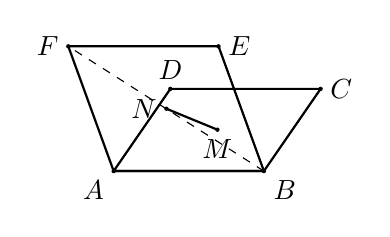
\begin{tikzpicture}[>=stealth,scale=0.72]
  \coordinate (A) at (0,0);
  \coordinate (B) at (2.65,0);
  \coordinate (C) at (3.65,1.45);
  \coordinate (D) at (1.0,1.45);
  \coordinate (E) at (1.85,2.20);
  \coordinate (F) at (-0.80,2.20);
  \coordinate (M) at (1.83,0.73);
  \coordinate (N) at (0.93,1.10);
  \draw[thick] (A)--(B)--(C)--(D)--cycle;
  \draw[thick] (A)--(B)--(E)--(F)--cycle;
  \draw[dashed] (A)--(D) (B)--(F);
  \draw[thick] (M)--(N);
  \fill (A) circle (1.1pt) node[below left] {$A$};
  \fill (B) circle (1.1pt) node[below right] {$B$};
  \fill (C) circle (1.1pt) node[right] {$C$};
  \fill (D) circle (1.1pt) node[above] {$D$};
  \fill (E) circle (1.1pt) node[right] {$E$};
  \fill (F) circle (1.1pt) node[left] {$F$};
  \fill (M) circle (1.1pt) node[below] {$M$};
  \fill (N) circle (1.1pt) node[left] {$N$};
\end{tikzpicture}
